\documentclass{oblivoir}
%%%Default packages
\usepackage{amsmath,amssymb,amsthm,kotex,tabu,graphicx,pifont}
\usepackage{../kswrapfig}

\usepackage{gensymb} %\degree

%%%More packages
%\usepackage{caption,subcaption}
%\usepackage[perpage]{footmisc}
%
\usepackage[skipabove=10pt,innertopmargin=10pt,nobreak=true]{mdframed}

\usepackage[inline]{enumitem}
\setlist[enumerate,1]{label=(\arabic*)}
\setlist[enumerate,2]{label=(\alph*)}

\usepackage{multicol}
\setlength{\columnsep}{30pt}
\setlength{\columnseprule}{1pt}
%
%\usepackage{forest}
%\usetikzlibrary{shapes.geometric,arrows.meta,calc}
%
%%%defi theo exam prob rema proo
%이 환경들 아래에 문단을 쓸 경우 살짝 들여쓰기가 되므로 \hspace{-.7em}가 필요할 수 있다.

\newcounter{num}
\newcommand{\defi}[1]
{\noindent\refstepcounter{num}\textbf{정의 \arabic{num})} #1\par\noindent}
\newcommand{\theo}[1]
{\noindent\refstepcounter{num}\textbf{정리 \arabic{num})} #1\par\noindent}
\newcommand{\revi}[1]
{\noindent\refstepcounter{num}\textbf{복습 \arabic{num})} #1\par\noindent}
\newcommand{\exam}[1]
{\bigskip\bigskip\noindent\refstepcounter{num}\textbf{예시 \arabic{num})} #1\par\noindent}
\newcommand{\prob}[1]
{\bigskip\bigskip\noindent\refstepcounter{num}\textbf{문제 \arabic{num})} #1\par\noindent}
\newcommand{\rema}[1]
{\bigskip\bigskip\noindent\refstepcounter{num}\textbf{참고 \arabic{num})} #1\par\noindent}
\newcommand{\proo}
{\bigskip\noindent\textsf{증명)}}

\newenvironment{talign}
 {\let\displaystyle\textstyle\align}
 {\endalign}
\newenvironment{talign*}
 {\let\displaystyle\textstyle\csname align*\endcsname}
 {\endalign}
%
%%%Commands

\newcommand{\procedure}[1]{\begin{mdframed}\vspace{#1\textheight}\end{mdframed}}

\newcommand\an[1]{\par\bigskip\noindent\textbf{문제 \ref{#1})}\par\noindent}

\newcommand\ann[2]{\par\bigskip\noindent\textbf{문제 \ref{#1})}\:\:#2\par\medskip\noindent}

\newcommand\ans[1]{\begin{flushright}\textbf{답 : }#1\end{flushright}}

\newcommand\anssec[1]{\bigskip\bigskip\noindent{\large\bfseries#1}}

\newcommand{\pb}[1]%\Phantom + fBox
{\fbox{\phantom{\ensuremath{#1}}}}

\newcommand\ba{\,|\,}

\newcommand\ovv[1]{\ensuremath{\overline{#1}}}
\newcommand\ov[2]{\ensuremath{\overline{#1#2}}}
%
%%%% Settings
%\let\oldsection\section
%
%\renewcommand\section{\clearpage\oldsection}
%
%\let\emph\textsf
%
%\renewcommand{\arraystretch}{1.5}
%
%%%% Footnotes
%\makeatletter
%\def\@fnsymbol#1{\ensuremath{\ifcase#1\or
%*\or **\or ***\or
%\star\or\star\star\or\star\star\star\or
%\dagger\or\dagger\dagger\or\dagger\dagger\dagger
%\else\@ctrerr\fi}}
%
%\renewcommand{\thefootnote}{\fnsymbol{footnote}}
%\makeatother
%
%\makeatletter
%\AtBeginEnvironment{mdframed}{%
%\def\@fnsymbol#1{\ensuremath{\ifcase#1\or
%*\or **\or ***\or
%\star\or\star\star\or\star\star\star\or
%\dagger\or\dagger\dagger\or\dagger\dagger\dagger
%\else\@ctrerr\fi}}%
%}   
%\renewcommand\thempfootnote{\fnsymbol{mpfootnote}}
%\makeatother
%
%%% 객관식 선지
\newcommand\one{\ding{172}}
\newcommand\two{\ding{173}}
\newcommand\three{\ding{174}}
\newcommand\four{\ding{175}}
\newcommand\five{\ding{176}}
\usepackage{tabto,pifont}
%\TabPositions{0.2\textwidth,0.4\textwidth,0.6\textwidth,0.8\textwidth}

\newcommand\taba[5]{\par\noindent
\one\:{#1}
\tabto{0.2\textwidth}\two\:\:{#2}
\tabto{0.4\textwidth}\three\:\:{#3}
\tabto{0.6\textwidth}\four\:\:{#4}
\tabto{0.8\textwidth}\five\:\:{#5}}

\newcommand\tabb[5]{\par\noindent
\one\:{#1}
\tabto{0.33\textwidth}\two\:\:{#2}
\tabto{0.67\textwidth}\three\:\:{#3}\medskip\par\noindent
\four\:\:{#4}
\tabto{0.33\textwidth}\five\:\:{#5}}

\newcommand\tabc[5]{\par\noindent
\one\:{#1}
\tabto{0.5\textwidth}\two\:\:{#2}\medskip\par\noindent
\three\:\:{#3}
\tabto{0.5\textwidth}\four\:\:{#4}\medskip\par\noindent
\five\:\:{#5}}

\newcommand\tabd[5]{\par\noindent
\one\:{#1}\medskip\par\noindent
\two\:\:{#2}\medskip\par\noindent
\three\:\:{#3}\medskip\par\noindent
\four\:\:{#4}\medskip\par\noindent
\five\:\:{#5}}
%
%%%% fonts
%
%\usepackage{fontspec, xunicode, xltxtra}
%\setmainfont[]{은 바탕}
%\setsansfont[]{은 돋움}
%\setmonofont[]{은 바탕}
%\XeTeXlinebreaklocale "ko"
\usepackage{fapapersize}
\usefapapersize{210mm,297mm,40mm,*,20mm,*}
\DeclareSymbolFont{yhlargesymbols}{OMX}{yhex}{m}{n}
\DeclareMathAccent{\wideparen}{\mathord}{yhlargesymbols}{"F3}
\usepackage{multirow,multicol}
%%%%
\begin{document}

\begin{center}
{\Large 신비, 미니테스트 3}
\end{center}

%
\prob{각도 \(\theta\)의 동경을 \(OP\)라고 할 때, \(P=(2,1)\)이다.}\label{property4}
\par\noindent
\begin{minipage}{.5\textwidth}
\begin{talign*}
\sin\theta&=\frac1{\sqrt5}\\
\cos\theta&=\frac2{\sqrt5}\\
\tan\theta&=\frac12
\end{talign*}
\end{minipage}
\begin{minipage}{.5\textwidth}
\vspace{10pt}
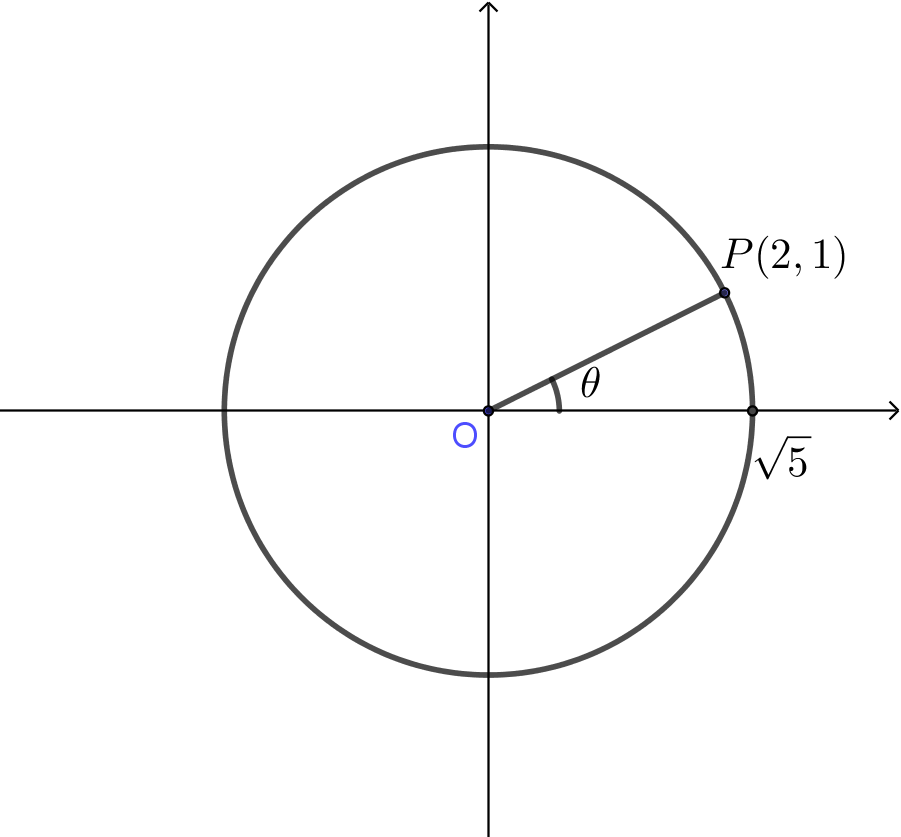
\includegraphics[width=.5\textwidth]{property_4}
\vspace{10pt}
\end{minipage}
\noindent
이때 다음 각도들에 대한 삼각비의 값을 차례로 구하여라.\\[10pt]
\begin{enumerate*}[itemjoin=\qquad\qquad]
\item
\(\theta-2\pi\)
\item
\(-\theta\)
\item
\(\theta-\pi\)
\item
\(\frac\pi2-\theta\)
\end{enumerate*}

\begin{enumerate}
\item
\begin{minipage}{.5\textwidth}
\begin{talign*}
\sin(\theta-2\pi)=&\\
\cos(\theta-2\pi)=&\\
\tan(\theta-2\pi)=&\\
\end{talign*}
\end{minipage}
\begin{minipage}{.5\textwidth}
\vspace{10pt}
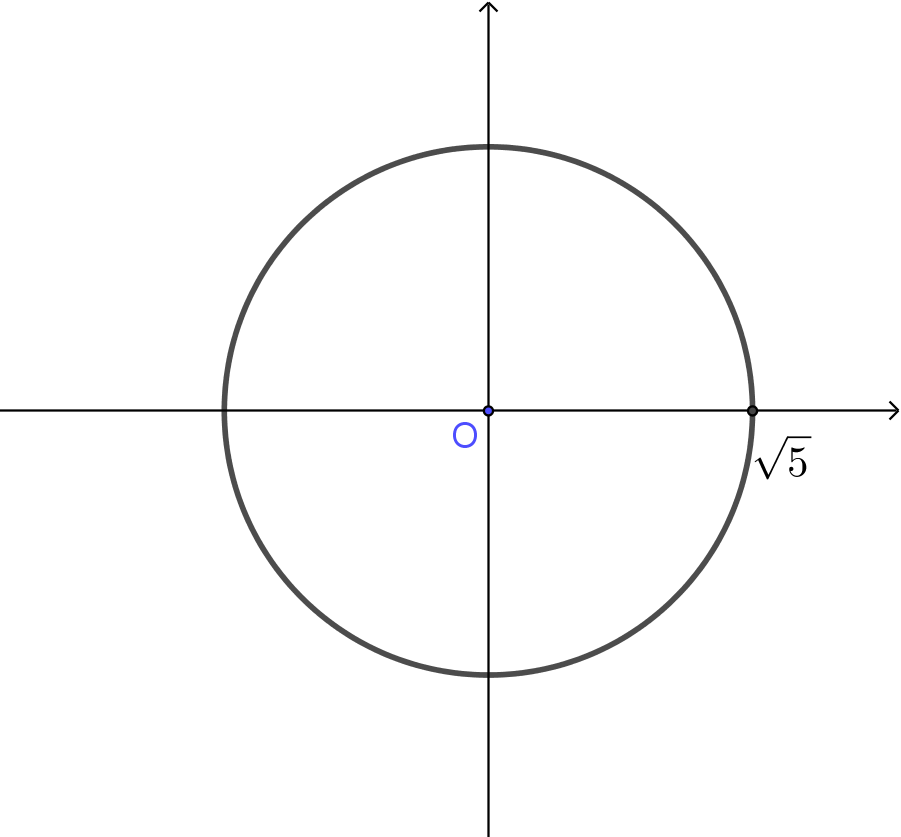
\includegraphics[width=.5\textwidth]{property_4-0}
\vspace{10pt}
\end{minipage}
\item
\begin{minipage}{.5\textwidth}
\begin{talign*}
\sin(-\theta)=&\\
\cos(-\theta)=&\\
\tan(-\theta)=&\\
\end{talign*}
\end{minipage}
\begin{minipage}{.5\textwidth}
\vspace{10pt}
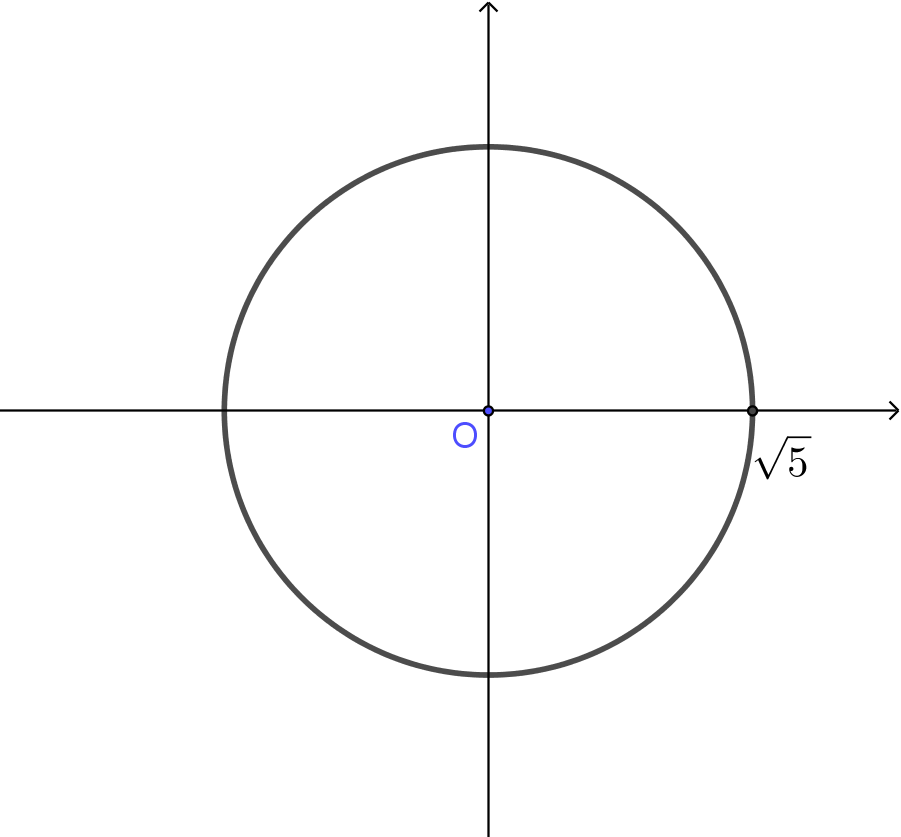
\includegraphics[width=.5\textwidth]{property_4-0}
\vspace{10pt}
\end{minipage}
\item
\begin{minipage}{.5\textwidth}
\begin{talign*}
\sin(\theta-\pi)=&\\
\cos(\theta-\pi)=&\\
\tan(\theta-\pi)=&\\
\end{talign*}
\end{minipage}
\begin{minipage}{.5\textwidth}
\vspace{10pt}
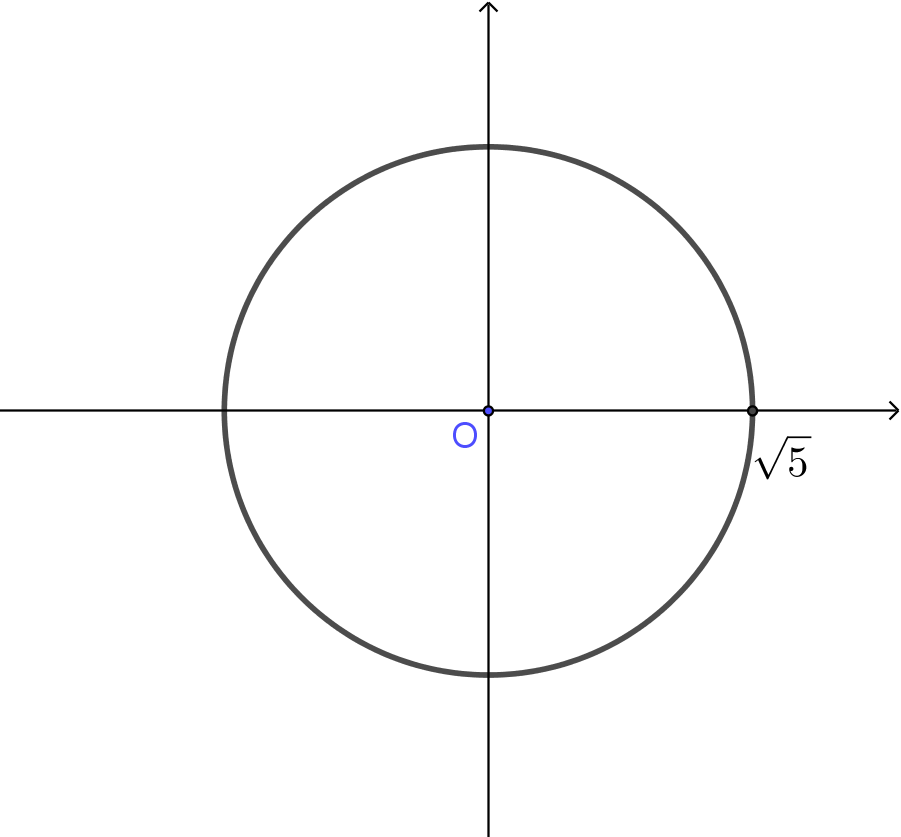
\includegraphics[width=.5\textwidth]{property_4-0}
\vspace{10pt}
\end{minipage}
\item
\begin{minipage}{.5\textwidth}
\begin{talign*}
\sin(\frac\pi2-\theta)=&\\
\cos(\frac\pi2-\theta)=&\\
\tan(\frac\pi2-\theta)=&\\
\end{talign*}
\end{minipage}
\begin{minipage}{.5\textwidth}
\vspace{10pt}
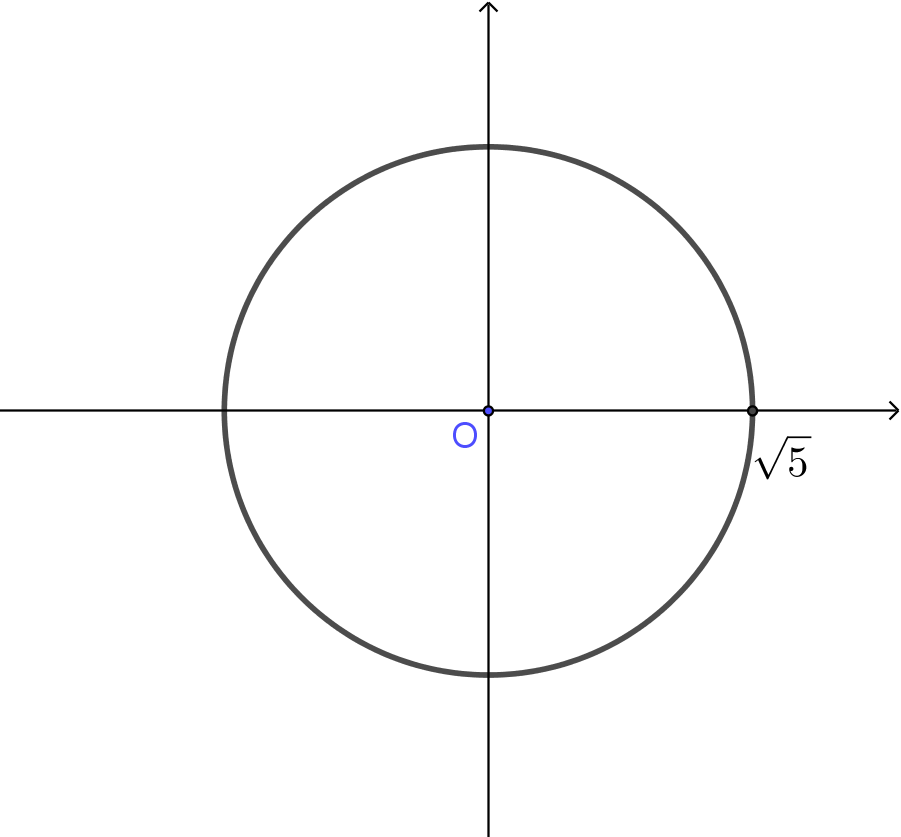
\includegraphics[width=.5\textwidth]{property_4-0}
\vspace{10pt}
\end{minipage}
\end{enumerate}

\newpage
%
\textbf{답 1)}
\begin{enumerate}
\item
\begin{minipage}{.5\textwidth}
\begin{talign*}
\sin(\theta-2\pi)=&\frac1{\sqrt5}\\
\cos(\theta-2\pi)=&\frac2{\sqrt5}\\
\tan(\theta-2\pi)=&\frac12\\
\end{talign*}
\end{minipage}
\begin{minipage}{.5\textwidth}
\vspace{10pt}
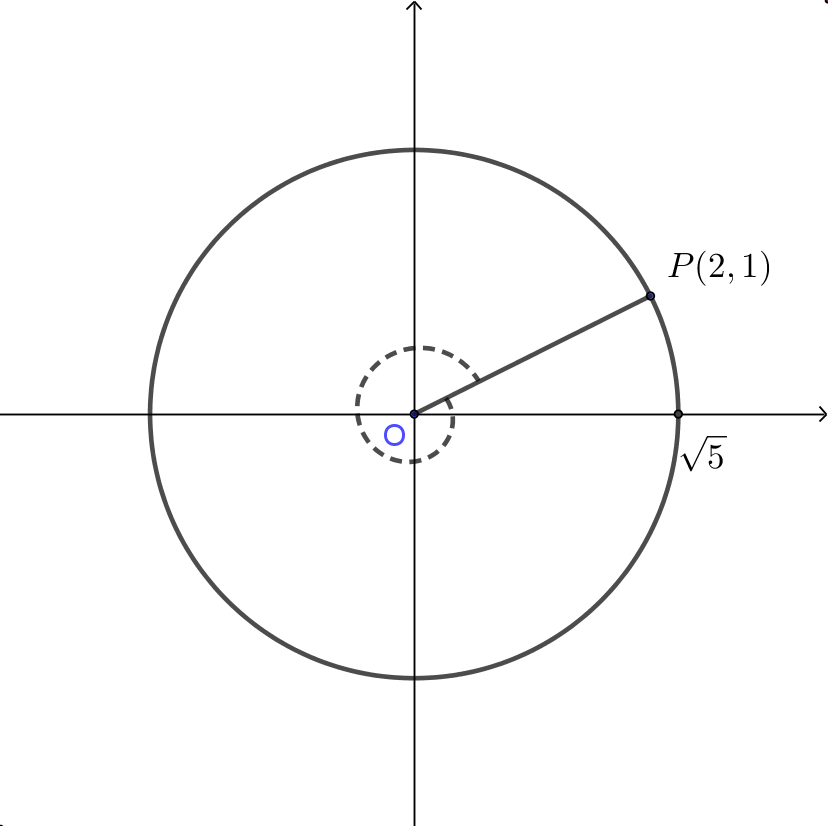
\includegraphics[width=.5\textwidth]{property_4-1}
\vspace{10pt}
\end{minipage}
\item
\begin{minipage}{.5\textwidth}
\begin{talign*}
\sin(-\theta)=&-\frac1{\sqrt5}\\
\cos(-\theta)=&\frac2{\sqrt5}\\
\tan(-\theta)=&-\frac12\\
\end{talign*}
\end{minipage}
\begin{minipage}{.5\textwidth}
\vspace{10pt}
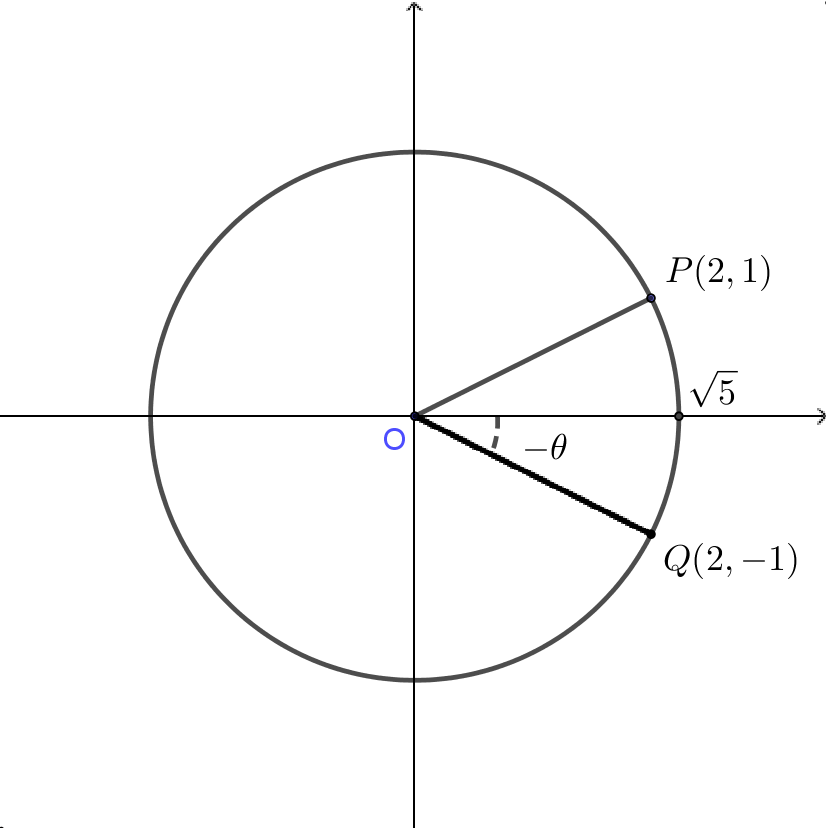
\includegraphics[width=.5\textwidth]{property_4-2}
\vspace{10pt}
\end{minipage}
\item
\begin{minipage}{.5\textwidth}
\begin{talign*}
\sin(\theta-\pi)=&-\frac1{\sqrt5}\\
\cos(\theta-\pi)=&-\frac2{\sqrt5}\\
\tan(\theta-\pi)=&\frac12\\
\end{talign*}
\end{minipage}
\begin{minipage}{.5\textwidth}
\vspace{10pt}
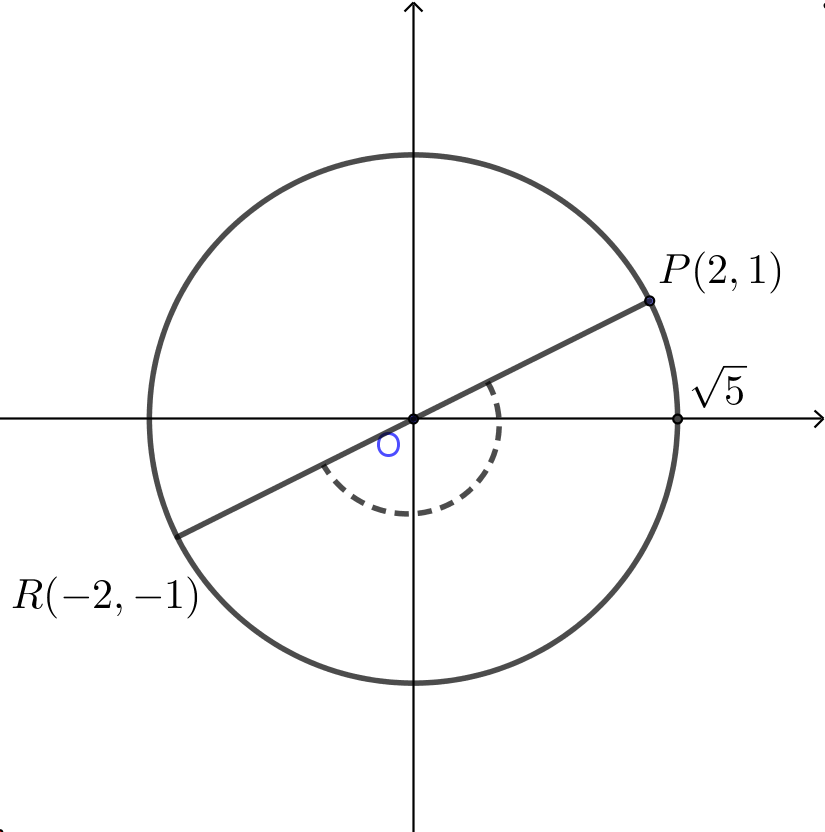
\includegraphics[width=.5\textwidth]{property_4-3}
\vspace{10pt}
\end{minipage}
\item
\begin{minipage}{.5\textwidth}
\begin{talign*}
\sin(\frac\pi2-\theta)=&\frac2{\sqrt5}\\
\cos(\frac\pi2-\theta)=&\frac1{\sqrt5}\\
\tan(\frac\pi2-\theta)=&2\\
\end{talign*}
\end{minipage}
\begin{minipage}{.5\textwidth}
\vspace{10pt}
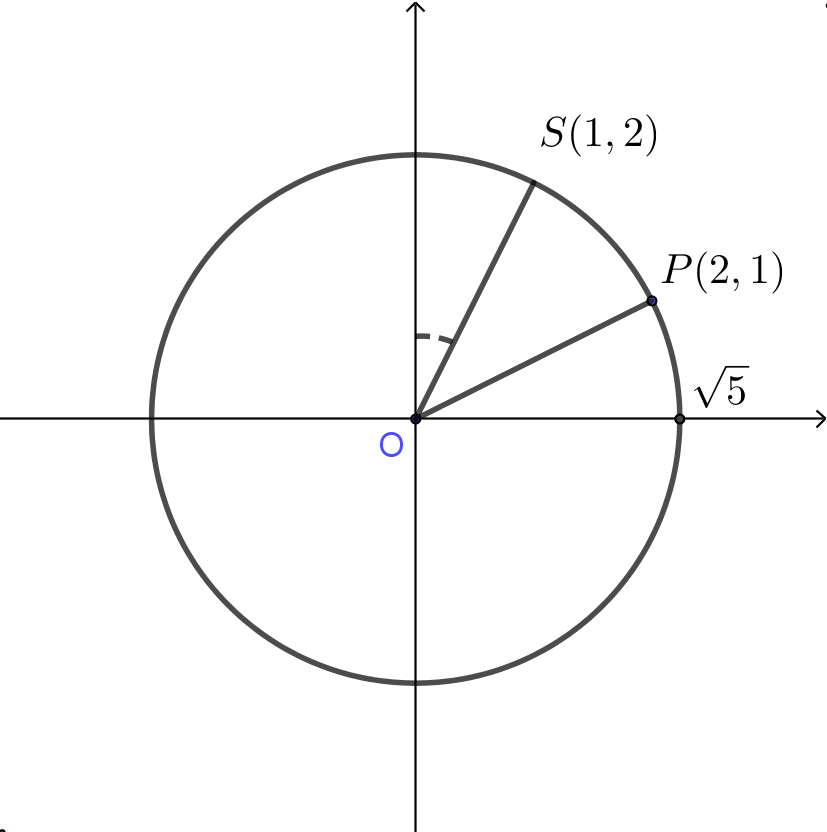
\includegraphics[width=.5\textwidth]{property_4-4}
\vspace{10pt}
\end{minipage}
\end{enumerate}

\end{document}